\chapter{Hardware description}\label{ch:hardware}
The Ethoscope is comprised of the following parts:
\begin{description}
  \item[Top unit] This contains the main components of the Ethoscope, such as the processing unit, the camera and the environmental monitor shield (optional). The components are enclosed in a plastic shell, as shown in figure~\ref{fig:case_top}.
    \begin{figure}
      \centering
      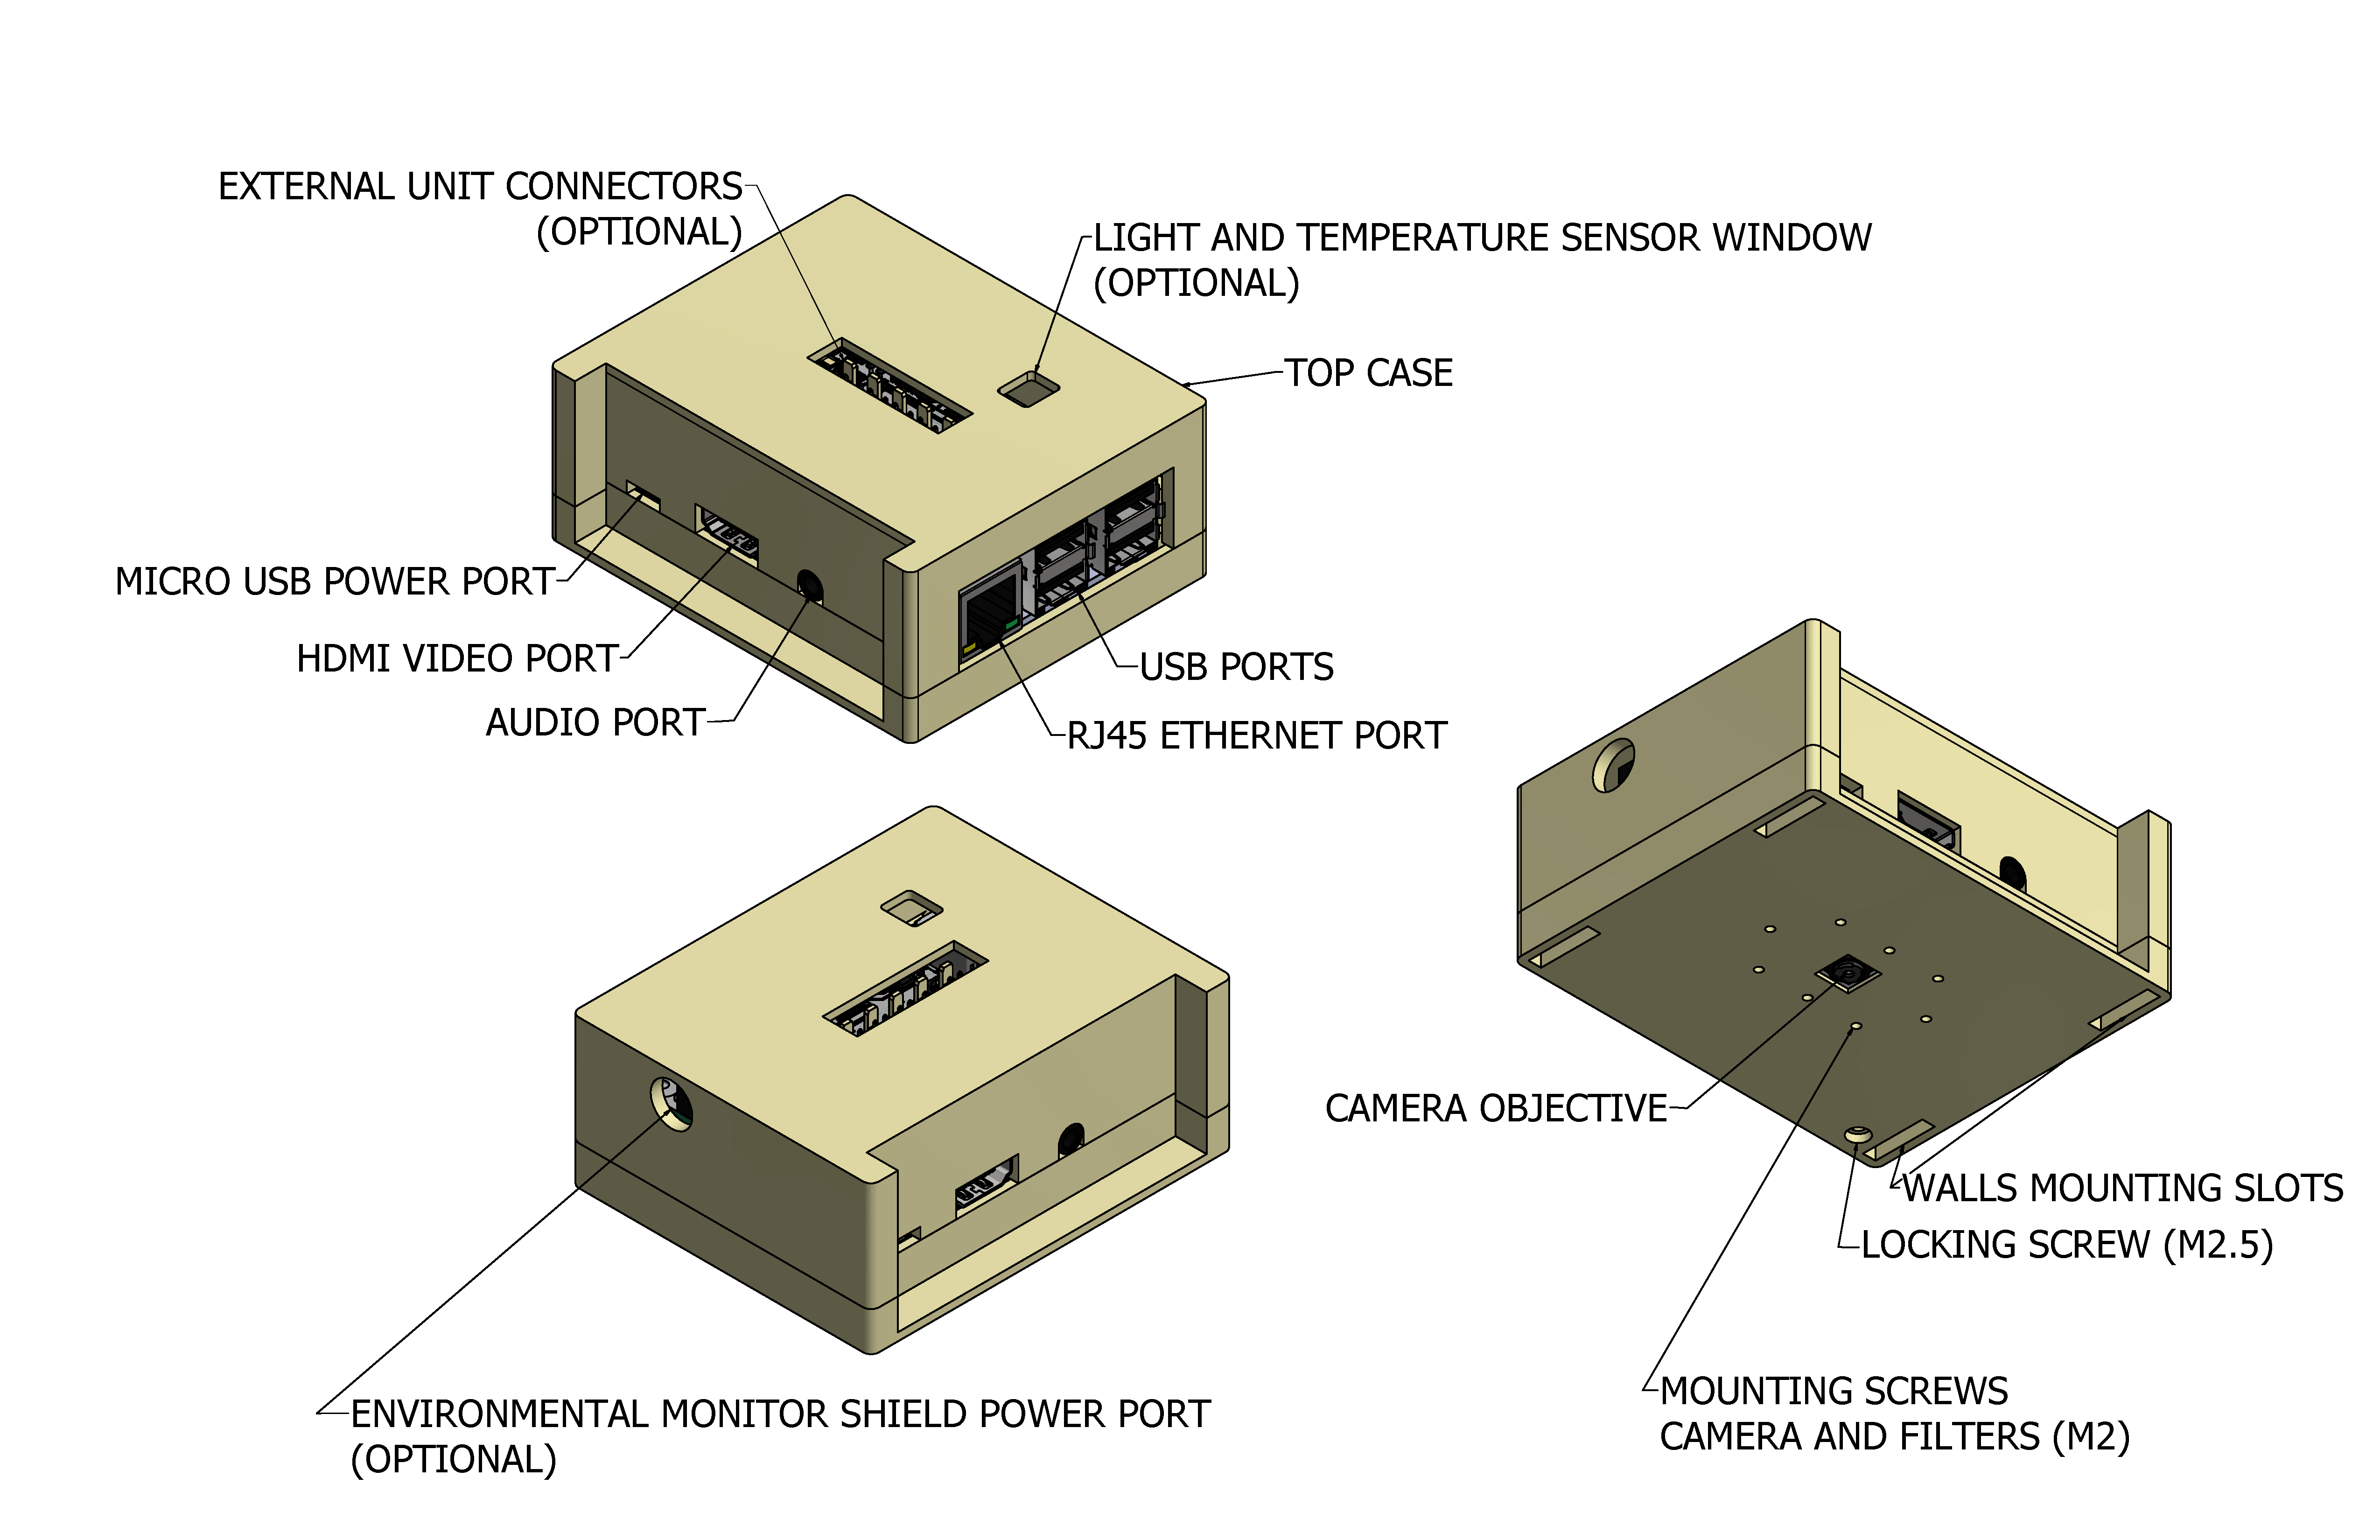
\includegraphics[width=0.9\textwidth]{./images/BasicComponentsTop.pdf}
      \caption{Top unit.}
      \label{fig:case_top}
    \end{figure}
      
  \item[Arena] The arena defines the experiment to be performed. The basic arena, provided with the standard kit, provides support for up to twenty glass tubes (figure~\ref{fig:basic_arena}; each tube defines a \gls{roi} within which a target can be tracked. Three black dots in the corner of the arena are used by the software to determine a system of reference.
    \begin{figure}
      \centering
      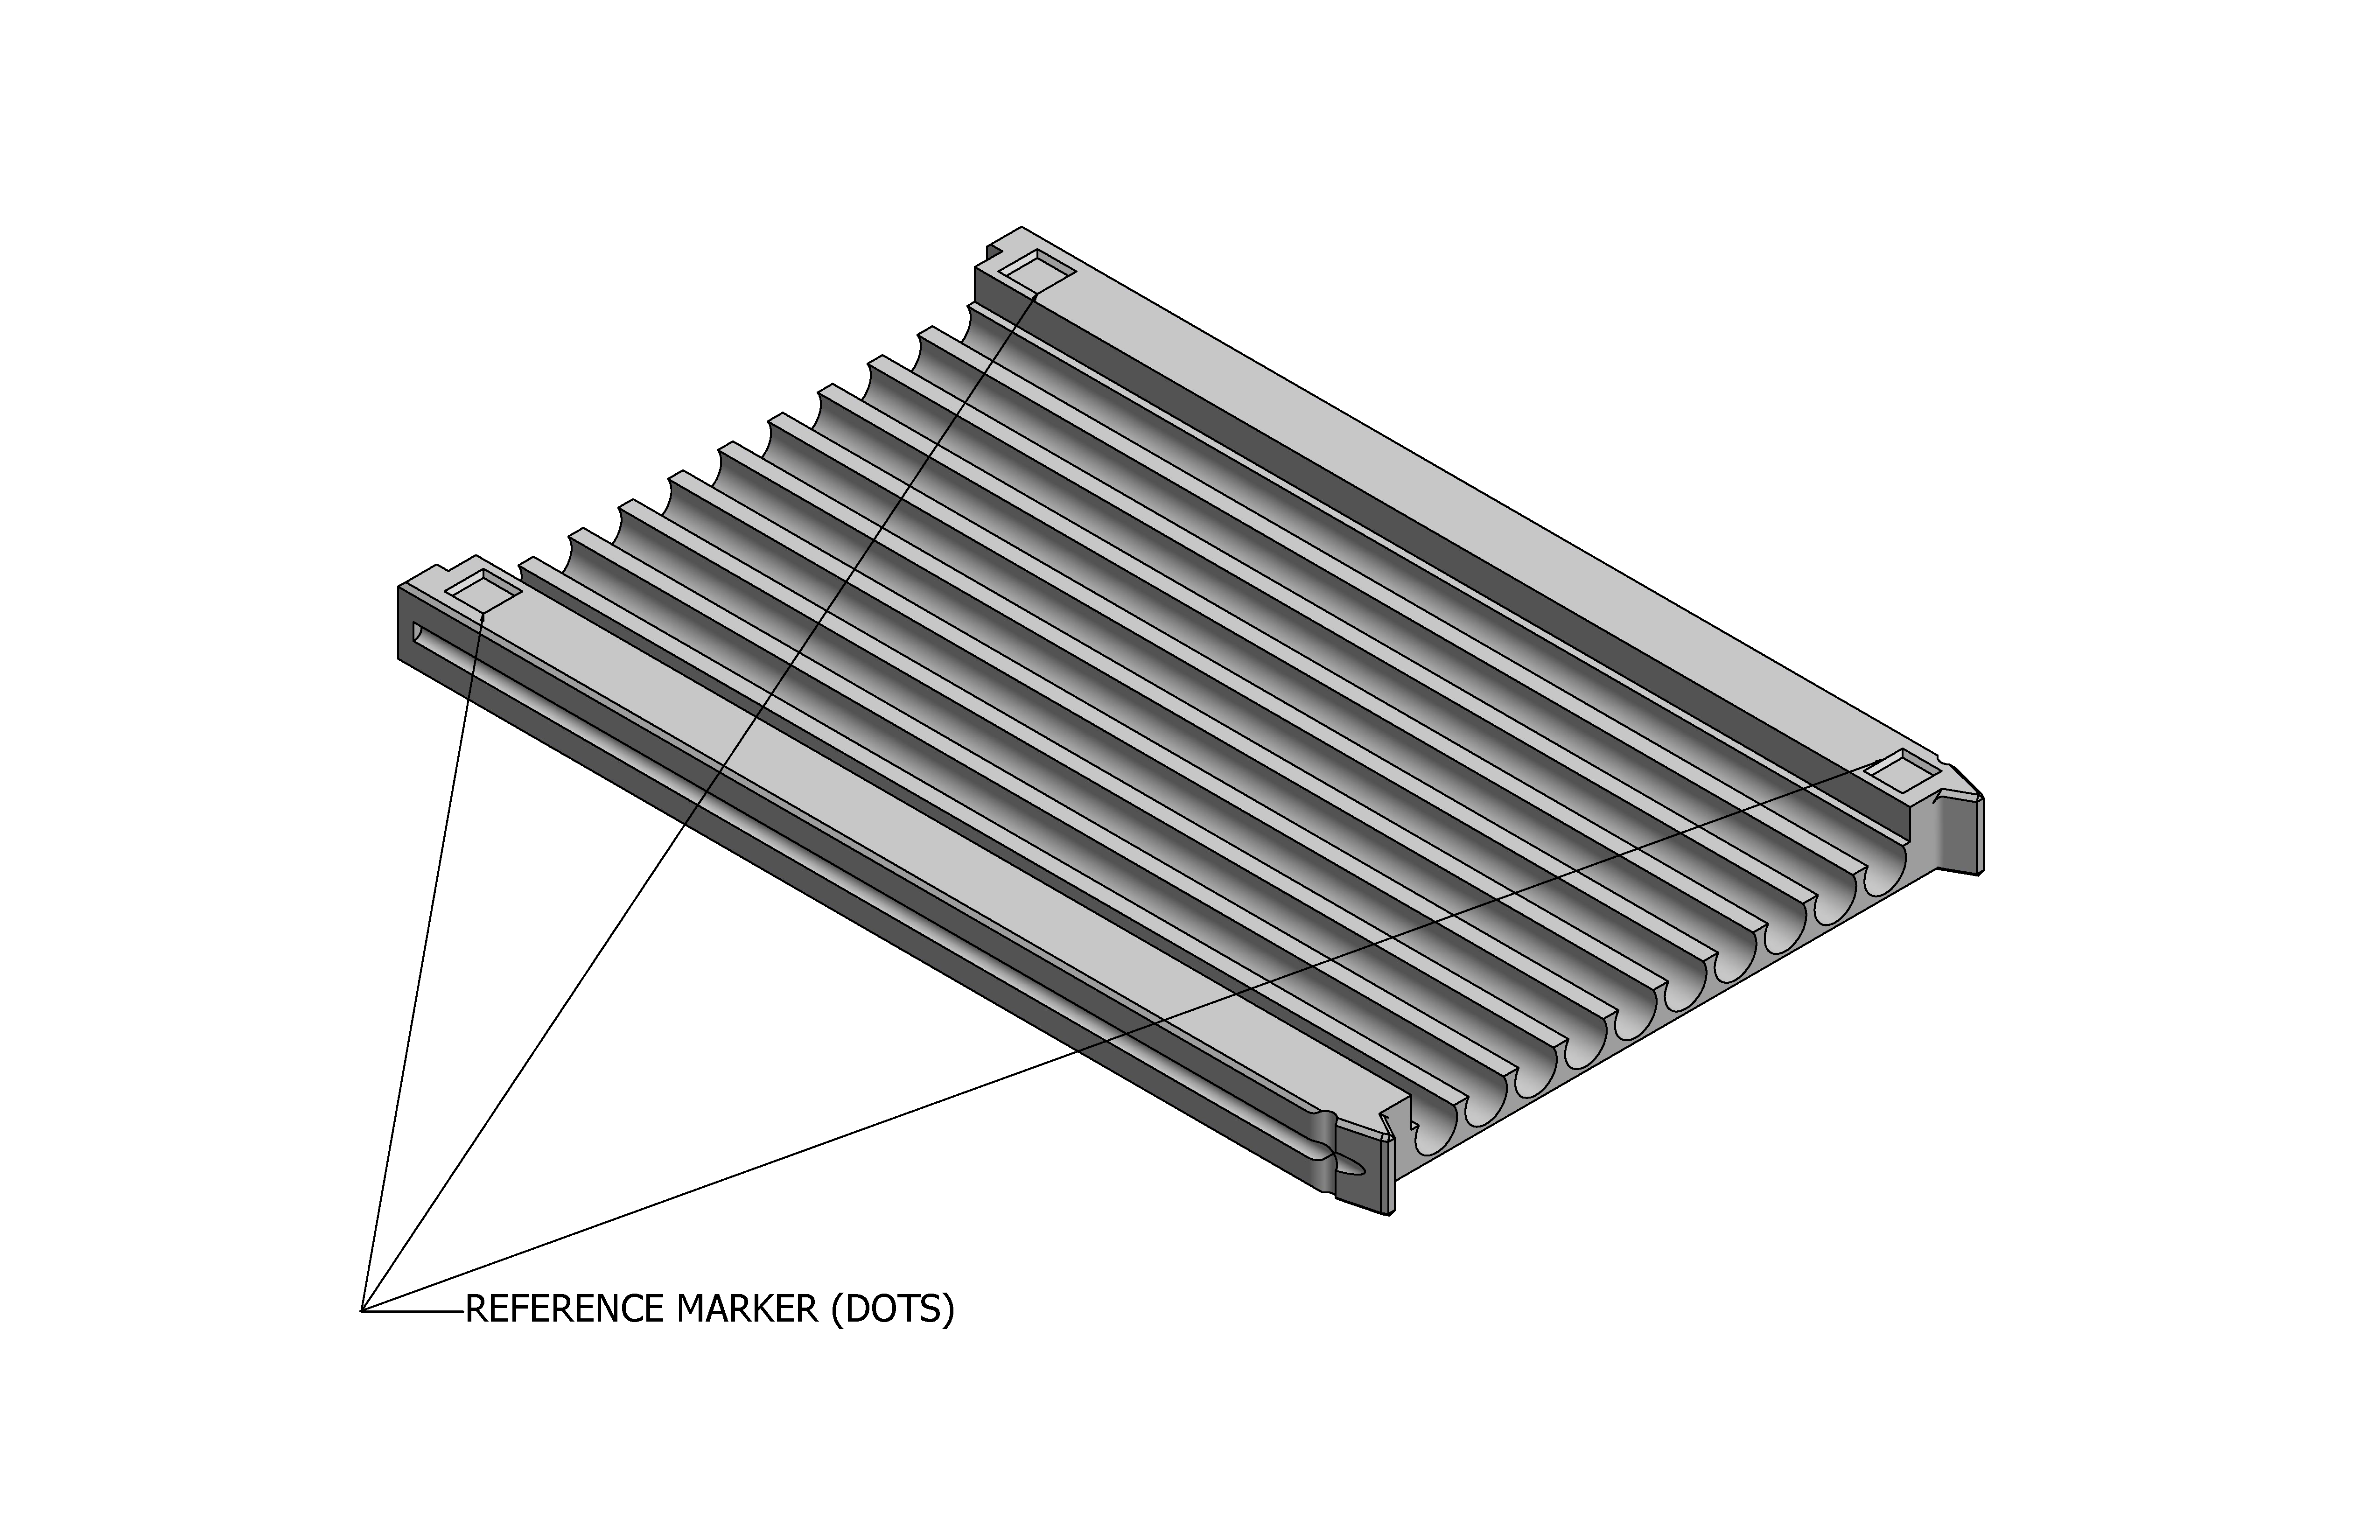
\includegraphics[width=0.8\textwidth]{./images/view_arena.pdf}
      \caption{The basic arena provided with the Ethoscope. Three black dots in the corners are used to provide alignment references to the software.}
      \label{fig:basic_arena}
    \end{figure}
    
  \item[Base unit] The unit (figure~\ref{fig:base_unit}) acts as a base for the whole Ethoscope and as a support and alignment tool for the arena. The base unit also contains the strip of \gls{led} used to provide \gls{ir} illumination to the arena. A slot in the side can be use to route wiring under the arena, for instance to install an optional vibrator unit.
    \begin{figure}
      \centering
      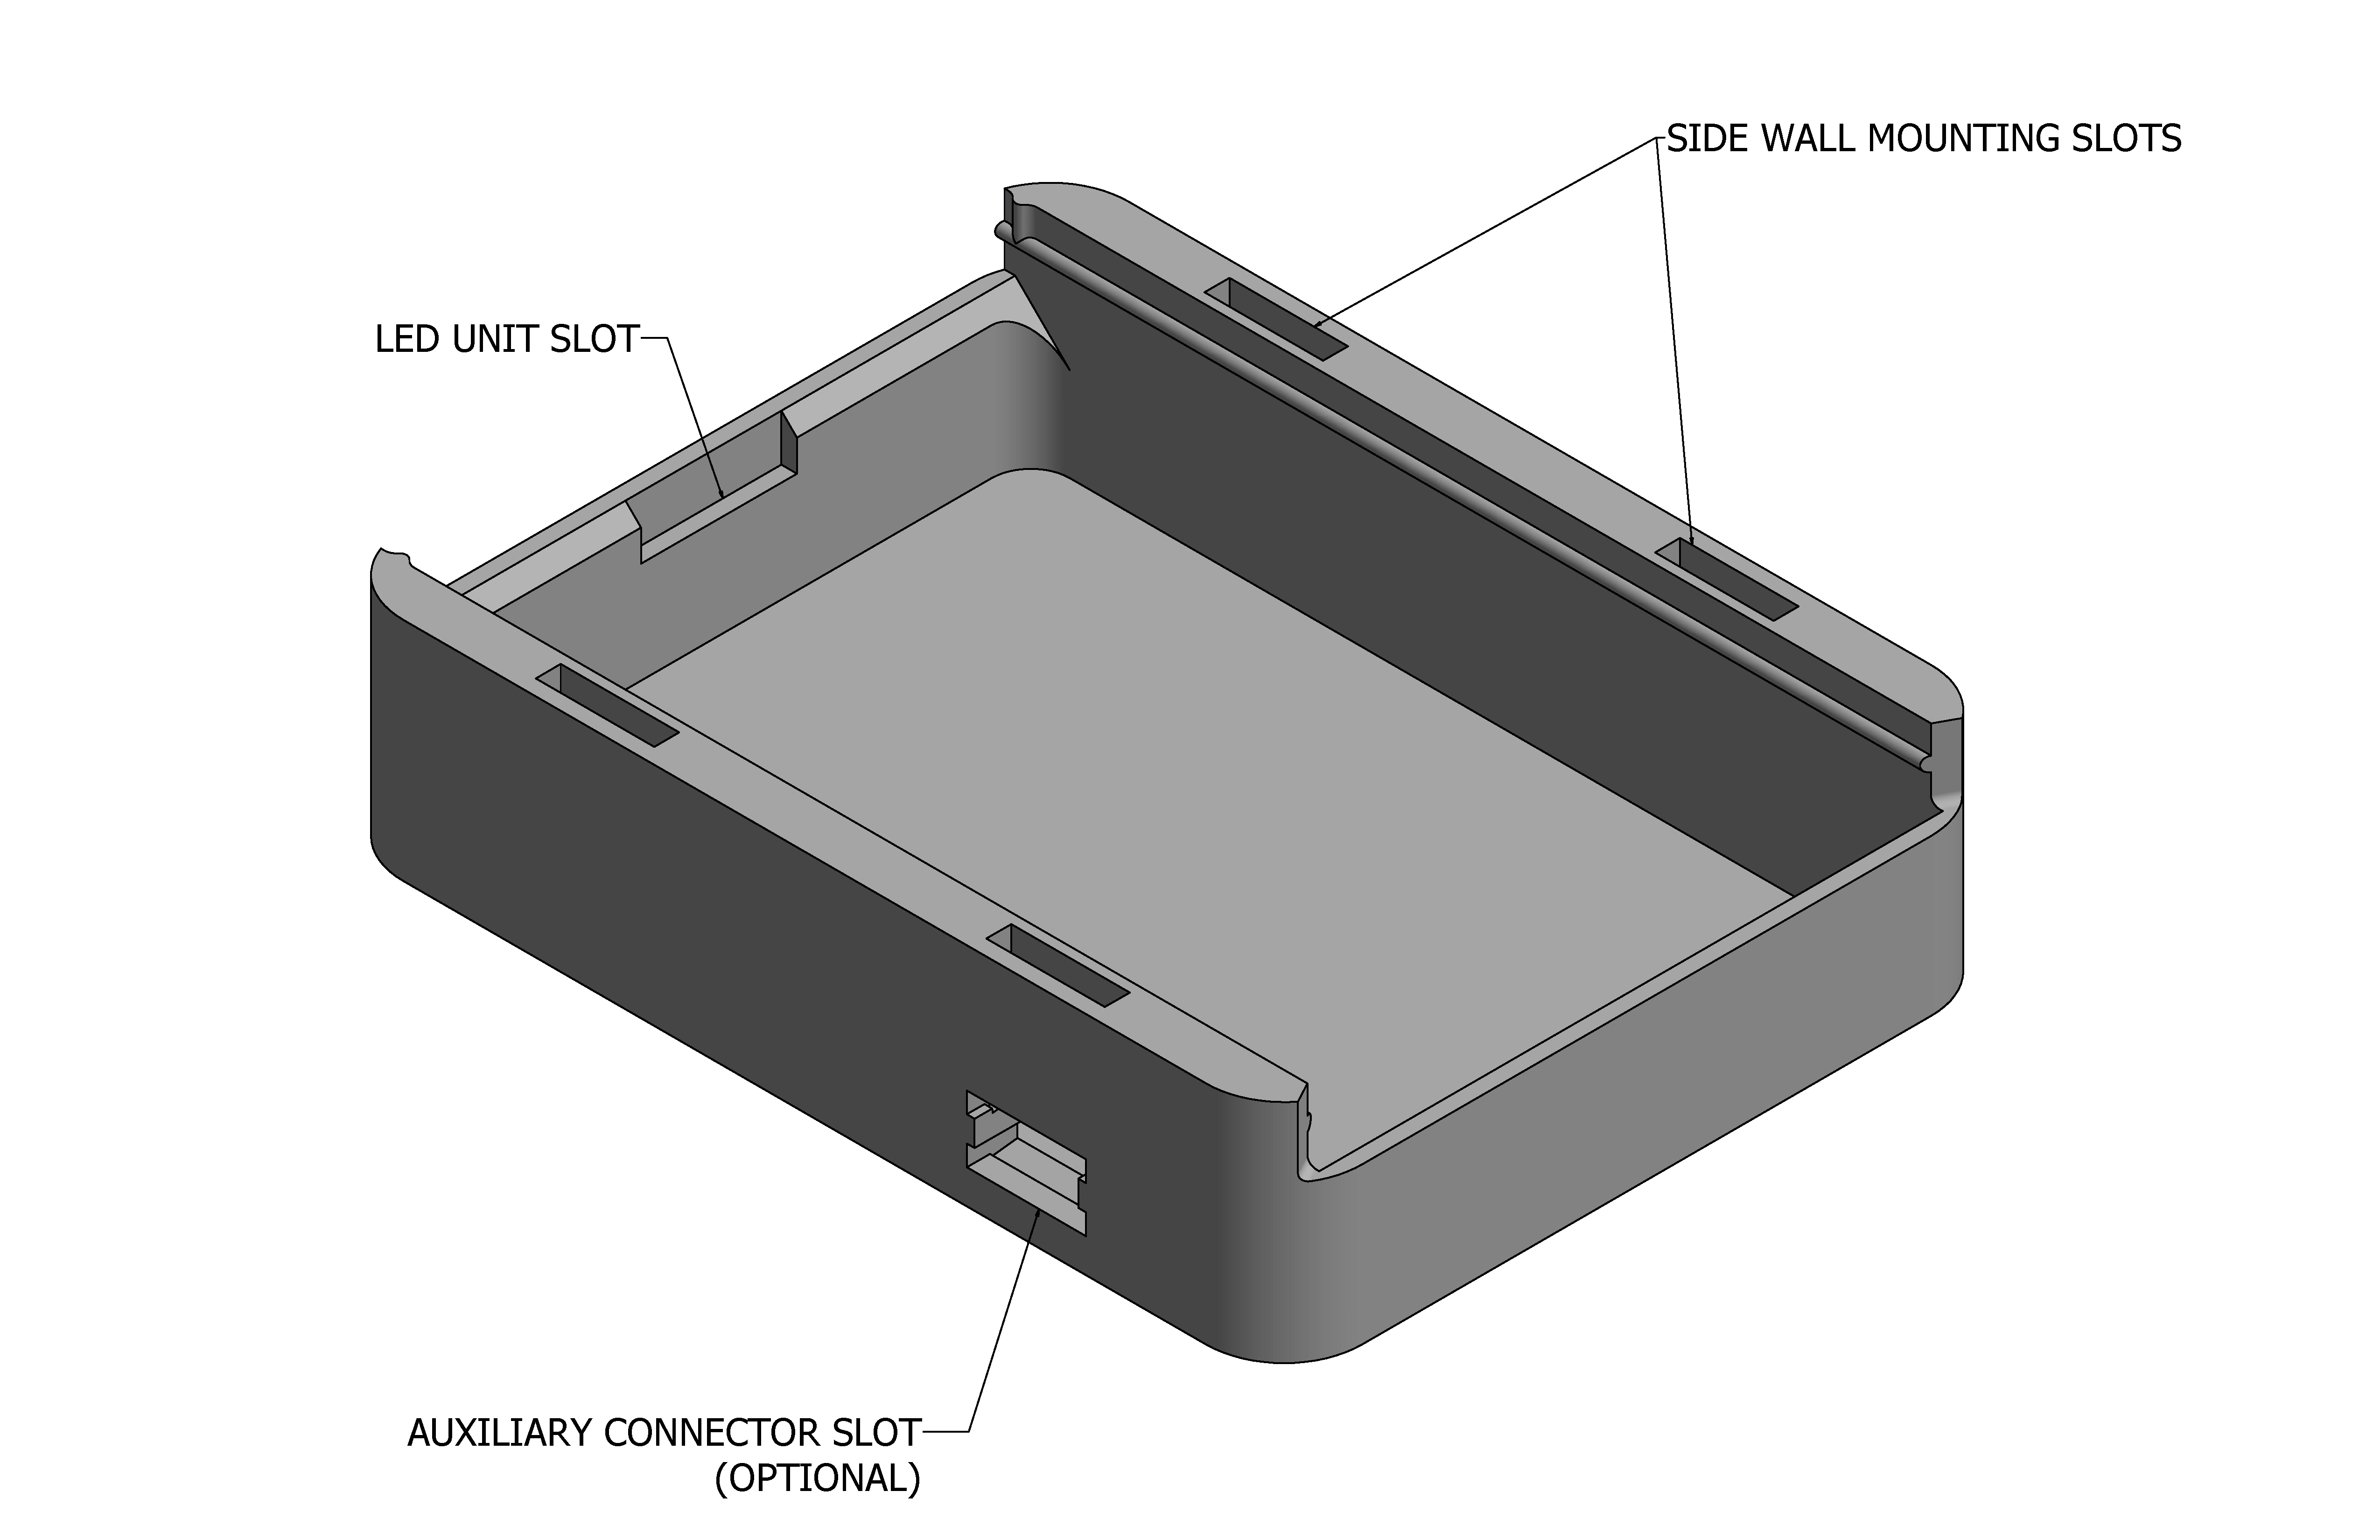
\includegraphics[width=0.8\textwidth]{./images/view_base.pdf}
      \caption{The basic arena provided with the Ethoscope. Three black dots in the corners are used to provide alignment references to the software.}
      \label{fig:base_unit}
    \end{figure}
      
  \item[Side walls] The walls connect the base to the top unit and ensure a correct distance between camera and arena. The standard walls are made of 3~mm acrylic sheet and are designed to ensure that the \gls{fov} of the camera covers the whole arena. 
\end{description}

\section{First setup}\label{ch:setup}
The following operations describe how to assemble and use the Ethoscope.
The top unit is shipped pre-assembled to reduce the number of operations required prior to using the Ethoscope.\\
If an additional component is purchased separately and needs to be installed, the unit can be taken apart by removing the M2.5 screw located at the bottom of the case and then opening the case to access the core electronics.
\begin{alertinfo}{WARNING}
        Be careful when disassembling and reassembling the unit. Do not force components; if in doubt contact Rymapt for assistance.\\
        The electronic components inside the Ethoscope can be damaged by \gls{esd}.\\
        Appropriate grounding is recommended whenever the electronic components are handled.
\end{alertinfo}\\
